\documentclass[11pt, a4paper]{report}

\usepackage[utf8]{inputenc}
\usepackage[margin=0.5in]{geometry}
\usepackage{fancyvrb}
\usepackage{amsmath}
\usepackage{amsfonts}
\usepackage{amssymb}
\usepackage{enumitem}
\usepackage{listings}
\usepackage{natbib}
\usepackage{amsmath, amsthm, amssymb}
\usepackage{ upgreek }
\usepackage{ tipa }
\usepackage{graphicx}

\begin{document}
\title{Practica04: Bifurcaciones}
\author{
  Introducci\'on a la Programaci\'on\\
  \texttt{19/Noviembre/2018}
  \and
  G\'omez Guti\'errez Uzziel\\
  \texttt{17-011-0019}
}
\date{}
\maketitle

\section*{Ejercicio 1}

\begin{figure}[!ht]
\begin{center}
  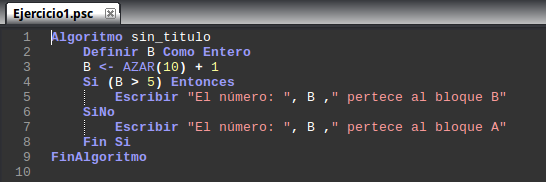
\includegraphics[width=0.8\textwidth]{ejercicio1.png}
  \caption{Pseudoc\'odigo ejercicio 1}
\end{center}
\end{figure}

\begin{figure}[!ht]
\begin{center}
  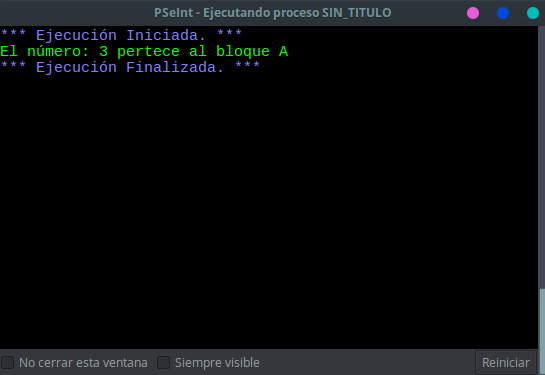
\includegraphics[width=0.5\textwidth]{respuesta1.png}
  \caption{El n\'umero se encuentra en la zona A.}
\end{center}
\end{figure}

\begin{figure}[!ht]
\begin{center}
  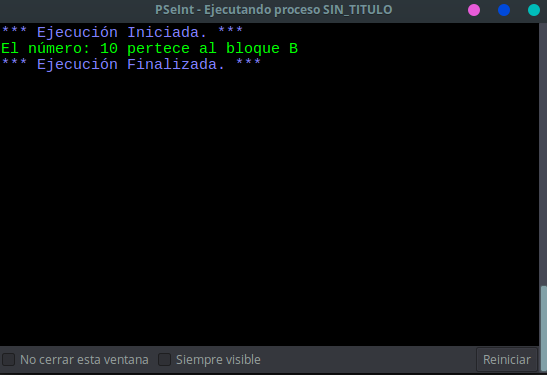
\includegraphics[width=0.5\textwidth]{respuesta2.png}
  \caption{El n\'umero se encuentra en la zona B.}
\end{center}
\end{figure}
 	
 \newpage	
\section*{Ejercicio 2}

\begin{figure}[!ht]
\begin{center}
  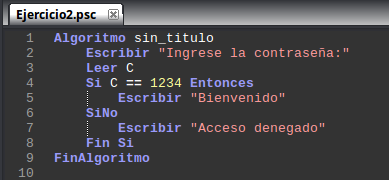
\includegraphics[width=0.7\textwidth]{ejercicio2.png}
  \caption{Pseudocodigo del ejercicio 2..}
\end{center}
\end{figure}

\begin{figure}[!ht]
\begin{center}
  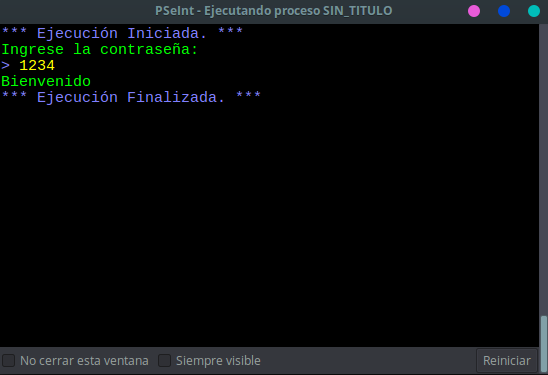
\includegraphics[width=0.5\textwidth]{respuesta3.png}
  \caption{Contraseña correcta.}
\end{center}
\end{figure}

\begin{figure}[!ht]
\begin{center}
  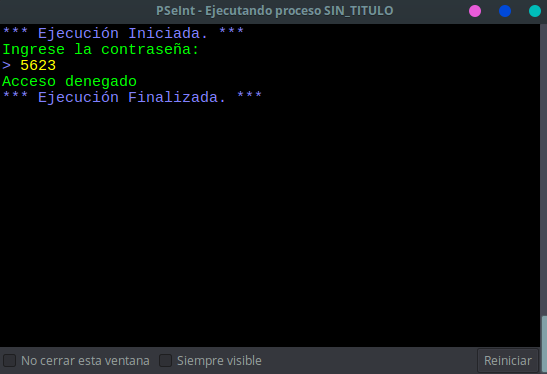
\includegraphics[width=0.5\textwidth]{respuesta4.png}
  \caption{Contraseña incorrecta.}
\end{center}
\end{figure}

\newpage
\section*{Ejercicio 3}

\begin{figure}[!ht]
\begin{center}
  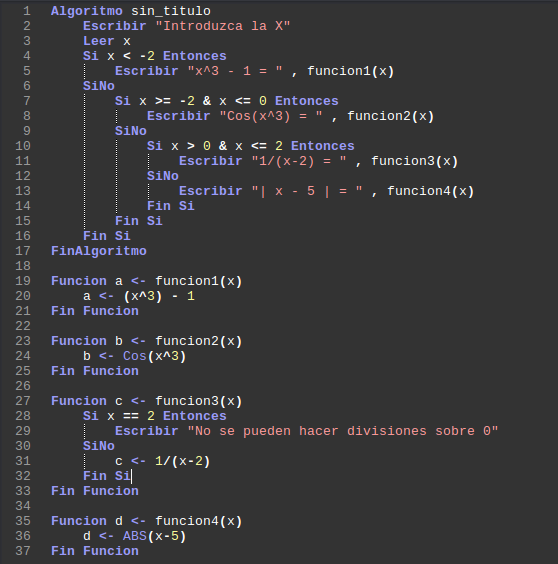
\includegraphics[width=0.7\textwidth]{ejercicio3.png}
  \caption{Pseudoc\'odigo ejercicio 3}
\end{center}
\end{figure}

\begin{figure}[!ht]
\begin{center}
  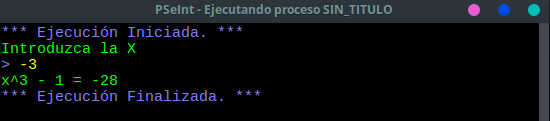
\includegraphics[width=0.6\textwidth]{respuesta5.png}
  \caption{Funci\'on evaluada en el primer intervalo.}
\end{center}
\end{figure} 

\begin{figure}[!ht]
\begin{center}
  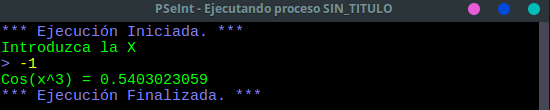
\includegraphics[width=0.6\textwidth]{respuesta6.png}
  \caption{Funci\'on evaluada en el segundo intervalo.}
\end{center}
\end{figure} 

\begin{figure}[!ht]
\begin{center}
  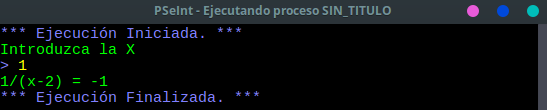
\includegraphics[width=0.6\textwidth]{respuesta7.png}
  \caption{Funci\'on evaluada en el tercer intervalo.}
\end{center}
\end{figure} 

\begin{figure}[!ht]
\begin{center}
  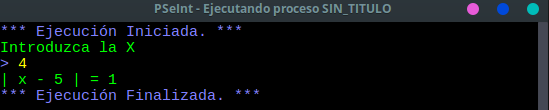
\includegraphics[width=0.6\textwidth]{respuesta9.png}
  \caption{Funci\'on evaluada en el cuarto intervalo.}
\end{center}
\end{figure} 

\begin{figure}[!ht]
\begin{center}
  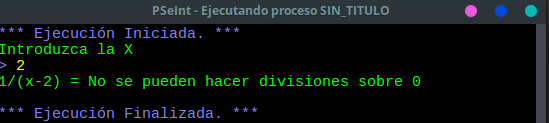
\includegraphics[width=0.6\textwidth]{respuesta8.png}
  \caption{Funci\'on evaluada en el cuarto intervalo cuando el divisor es 0.}
\end{center}
\end{figure} 

\newpage
\section*{Ejercicio 4}

\begin{figure}[!ht]
\begin{center}
  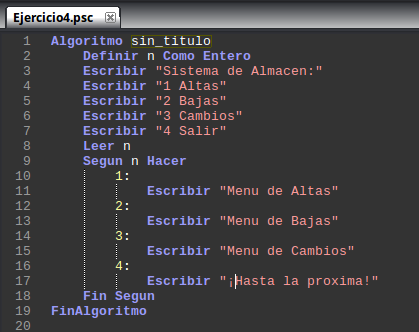
\includegraphics[width=0.6\textwidth]{ejercicio4.png}
  \caption{Pseudoc\'odigo ejercicio 4.}
\end{center}
\end{figure}

\begin{figure}[!ht]
\begin{center}
  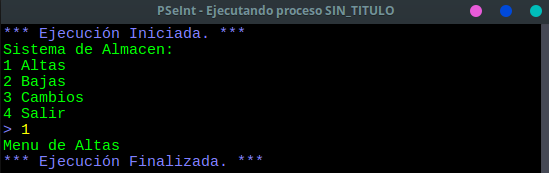
\includegraphics[width=0.6\textwidth]{respuesta10.png}
  \caption{Menu de Altas.}
\end{center}
\end{figure}

\begin{figure}[!ht]
\begin{center}
  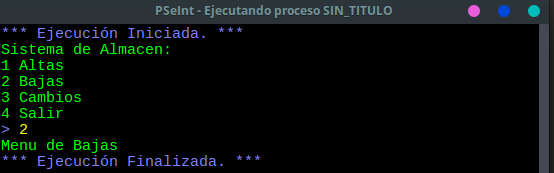
\includegraphics[width=0.6\textwidth]{respuesta11.png}
  \caption{Menu de Bajas.}
\end{center}
\end{figure} 

\begin{figure}[!ht]
\begin{center}
  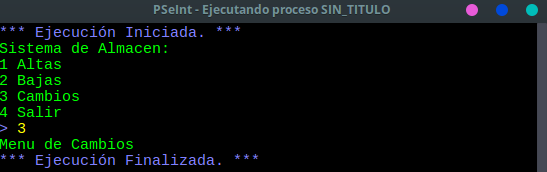
\includegraphics[width=0.6\textwidth]{respuesta12.png}
  \caption{Menu de Cambios.}
\end{center}
\end{figure} 

\begin{figure}[!ht]
\begin{center}
  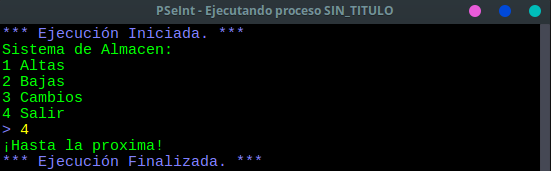
\includegraphics[width=0.6\textwidth]{respuesta13.png}
  \caption{Opci\'on Salir.}
\end{center}
\end{figure} 

\newpage
\section*{Ejercicio 5}

\begin{figure}[!ht]
\begin{center}
  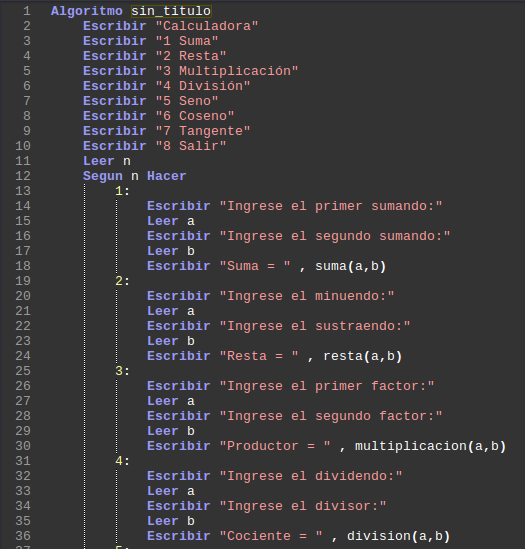
\includegraphics[width=0.7\textwidth]{ejercicio5.png}
  \caption{Pseudoc\'odigo ejercicio 5 (primera parte).}
\end{center}
\end{figure}

\begin{figure}[!ht]
\begin{center}
  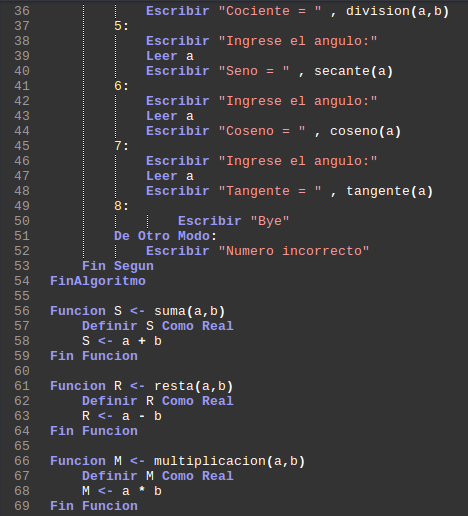
\includegraphics[width=0.7\textwidth]{ejercicio51.png}
  \caption{Pseudoc\'odigo ejercicio 5 (segunda parte).}
\end{center}
\end{figure}

\begin{figure}[!ht]
\begin{center}
  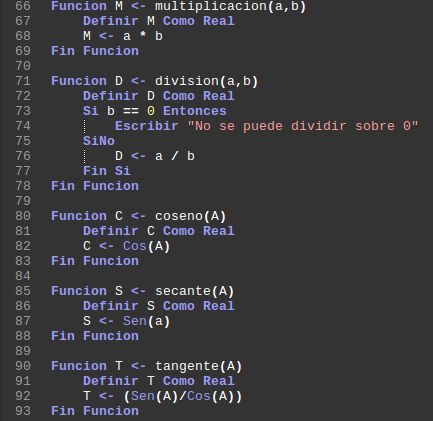
\includegraphics[width=0.7\textwidth]{ejercicio53.png}
  \caption{Pseudoc\'odigo ejercicio 5 (tercera parte).}
\end{center}
\end{figure}

\begin{figure}[!ht]
\begin{center}
  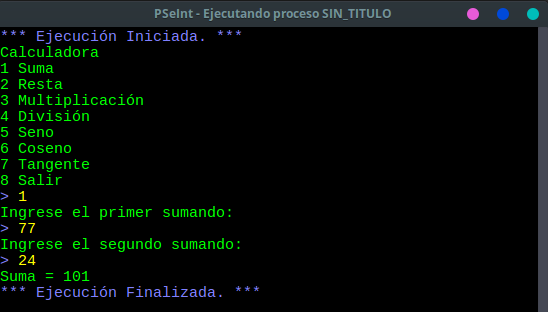
\includegraphics[width=0.6\textwidth]{respuesta14.png}
  \caption{Opci\'on suma.}
\end{center}
\end{figure}

\begin{figure}[!ht]
\begin{center}
  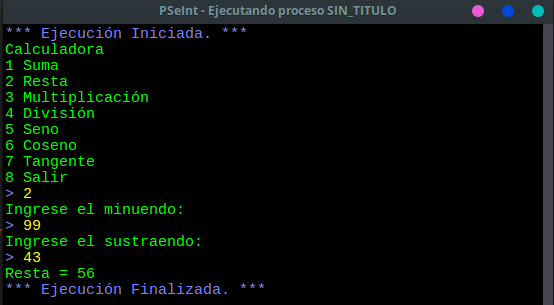
\includegraphics[width=0.6\textwidth]{respuesta15.png}
  \caption{Opci\'on resta.}
\end{center}
\end{figure}

\begin{figure}[!ht]
\begin{center}
  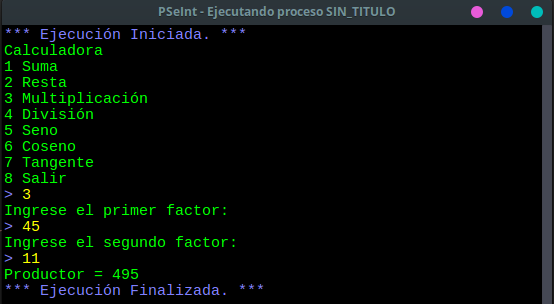
\includegraphics[width=0.6\textwidth]{respuesta16.png}
  \caption{Opci\'on multiplicaci\'on.}
\end{center}
\end{figure} 

\begin{figure}[!ht]
\begin{center}
  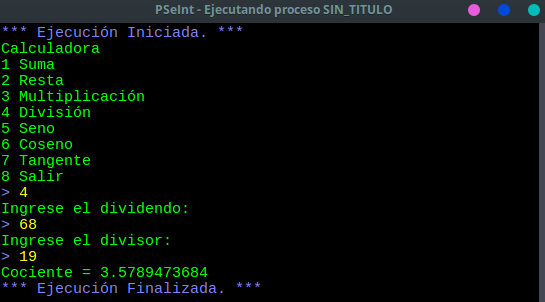
\includegraphics[width=0.6\textwidth]{respuesta17.png}
  \caption{Opci\'on divisi\'on.}
\end{center}
\end{figure} 

\begin{figure}[!ht]
\begin{center}
  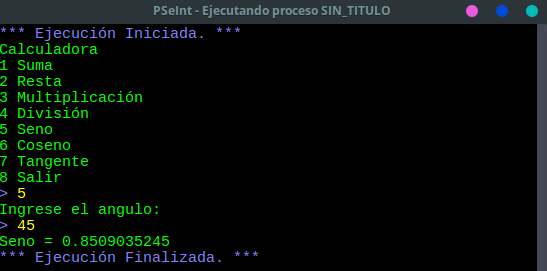
\includegraphics[width=0.6\textwidth]{respuesta18.png}
  \caption{Opci\'on funci\'on seno.}
\end{center}
\end{figure} 

\begin{figure}[!ht]
\begin{center}
  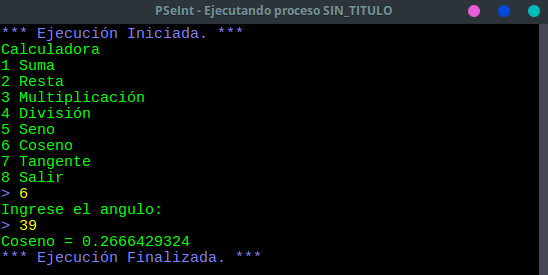
\includegraphics[width=0.6\textwidth]{respuesta19.png}
  \caption{Opci\'on funci\'on coseno.}
\end{center}
\end{figure}

\begin{figure}[!ht]
\begin{center}
  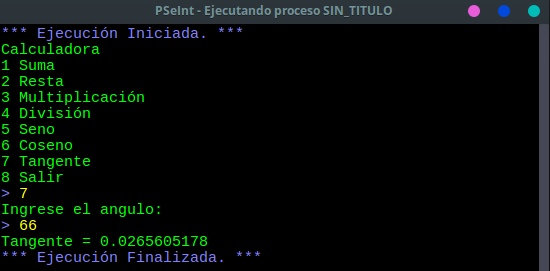
\includegraphics[width=0.6\textwidth]{respuesta20.png}
  \caption{Opci\'on funci\'on tangente.}
\end{center}
\end{figure} 

\begin{figure}[!ht]
\begin{center}
  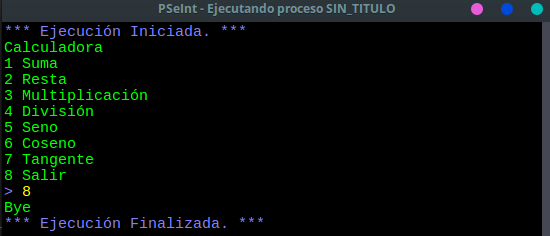
\includegraphics[width=0.6\textwidth]{respuesta21.png}
  \caption{Opci\'on salir.}
\end{center}
\end{figure} 
 

\end{document}